% ****** Start of file aipsamp.tex ******
%
%   This file is part of the AIP files in the AIP distribution for REVTeX 4.
%   Version 4.1 of REVTeX, October 2009
%
%   Copyright (c) 2009 American Institute of Physics.
%
%   See the AIP README file for restrictions and more information.
%
% TeX'ing this file requires that you have AMS-LaTeX 2.0 installed
% as well as the rest of the prerequisites for REVTeX 4.1
%
% It also requires running BibTeX. The commands are as follows:
%
%  1)  latex  aipsamp
%  2)  bibtex aipsamp
%  3)  latex  aipsamp
%  4)  latex  aipsamp
%
% Use this file as a source of example code for your aip document.
% Use the file aiptemplate.tex as a template for your document.
\documentclass[%
 aip,
 jmp,%
 amsmath,amssymb,
%preprint,%
 reprint,%
%author-year,%
%author-numerical,%
]{revtex4-1}

\usepackage{graphicx}% Include figure files
\usepackage{dcolumn}% Align table columns on decimal point
\usepackage{bm}% bold math
\usepackage{amssymb} 
%\usepackage[nomarkers,figuresonly]{endfloat}
%\usepackage[mathlines]{lineno}% Enable numbering of text and display math
%\linenumbers\relax % Commence numbering lines

\begin{document}

\title[Brain Network Study During Resting States]{Brain Network Study During Resting States\\}

\author{Mattia Podio}

\author{Konstantinos Sioumalas Christodolou}%

\author{Mattias Basso}

\date{\today}% It is always \today, today,
             %  but any date may be explicitly specified

\keywords{EEG data, brain network, connectivity graph, graph indices, motif analysis, community detection}%Use showkeys class option if keyword
                              %display desired
\maketitle


% \section{\label{sec:level1}First-level heading}
% \subsection{\label{sec:level2}Second-level heading}
% \subsubsection{\label{sec:level3}Third-level heading}

The goal of this project is to conduct some analysis on two datasets of EEG data. In this report we explain briefly what we did and we try to get some insight from the results of the analysis. For a complete list of the tasks completed, see Appendix A.

Data \cite{dataset} are taken from a public repository published from the Physionet Project. This data set consists of over 1500 one- and two-minute EEG recordings, obtained from 109 volunteers, but in our tasks we used just two runs from a specific subject (\verb|S001|): the first run - \verb|R01| - is recorded during eyes-open (EO) resting state, while the second one - \verb|R02| - is recorded during eyes-closed (EC) resting state.

Generally we worked in Python, so in order to read EEG data, that are stored in \verb|EDF| format we used the \verb|pyedflib| library \cite{pyedflib}

\section{\label{sec:level1}Connectivity Graphs}

In the last decades, a big effort has been made to apply graph theory to neuroscience. For that purpose we used some basic but important tools of graph theory to identify the brain connectivity of the previous resting states.

Graph theory provides powerful means to assess topology and organization of brain connectivity networks

A network based approach is especially useful when it's important to comprehend and highlight non obvious interactions between agents in a system, their nature depending on the case study. In computational neuroscience we measure the neuronal activity of different brain regions through sensors applied on top of the scalp. Functional connectivity can be estimated using methods based on Granger causality, such as multivariate autoregressive models (MVAR).

A multivariate autoregressive model of order $p$ can be defined as 

\begin{equation}
	X(t) = \sum_{r = 1}^{p} A(r)X(t-r) + E(t)
\end{equation}

In our case, $X(t)$ is a vector that contains measurements from 64 signals at time $t$; $A(r)$ $r\in \{1,2,..p\}$ are matrices in $\mathbb{R}^{N\times N}$ that contain the parameters (to be estimated) that describe the dependence between the entries in $X(t)$ and $X(t-r)$; $E(t)$ is a vector of random variables and denotes the uncorrelated Gaussian process with zero mean.

The formula says that values at time $t$ linearly depend from the last $p$ values taken from our 64 time series through an appropriate set of $N \cdot N \cdot p$ coefficients.\\

It is possible to select the best value of $p$ with respect to the Akaike information criterion. This selection required us to spend to much time on that, and since we considered this not crucial for our purposes, we set the order of the model to $p = 3$. Further investigations can surely be made in future studies.\cite{DengfengHuang}\\

What is written above can be rewritten also like.

\begin{equation}
	\sum_{r = 0}^{p} A(r)X(t-r) = E(t)
\end{equation}

if $A(0) = \mathbb{I}$, and $A(r)$ $r\in \{1,2,3\}$ are estimated by solving the Yule Walker equations. \\

EEG signals are both defined in time as well as in frequency. We are interested in the reconstruction of the direction of information flows in the network.

Applying the Fourier Transform to both sides, hence passing to the frequency domain we have these two results

\begin{equation}
A(f)X(f) = E(f)
\end{equation}

\begin{equation}
X(f) = A^{-1}(f)E(f) = H(f)E(f)
\end{equation}


Partial Directed Coherence - PDC - is defined as 

\begin{equation}
	\pi_{ij}(f) = \frac{|A_{ij}(f)|^2}{\sum_{m=1}^{N}|A_{mi}(f)|^2}
\end{equation}

Directed Fourier Transform - DTF - is defined as 

\begin{equation}
	\theta_{ij}(f) = \frac{|H_{ij}(f)|^2}{\sum_{m=1}^{N}|H_{mi}(f)|^2}
\end{equation}

Once we calculated these estimators, choosing a particular frequency $f^*$ we can effectively start using a graph formalism: in fact what we did is to construct a graph from using either $\pi(f^*)$ or $\theta(f^*)$.

We conduct the analysis below selecting the topology that arises choosing $f^* = \text{10 Hz}$; they basically corresponds to the alpha waves (8 – 12.5 Hz), that predominantly originate from the occipital lobe during wakeful relaxation with closed eyes. Alpha waves are reduced with open eyes, drowsiness and sleep\cite{alphaPalva}.

We also generate the graphs relative to $f^* = \text{28 Hz}$, i.e. to high beta waves (20.5–28 Hz); beta states are the states associated with normal waking consciousness \cite{betaWiki}.\\

When creating a graph object, we put a threshold on network density. Through a custom function we iteratively select the less meaningful edge - i.e. edge with the lowest weight - and we delete it, until criteria on the density is satisfied. In case of multiple edges with equal lowest weight, what the function does is to select one of them at random. Unless otherwise stated, we will refer to graphs with density d = 0.05.

\begin{figure}
	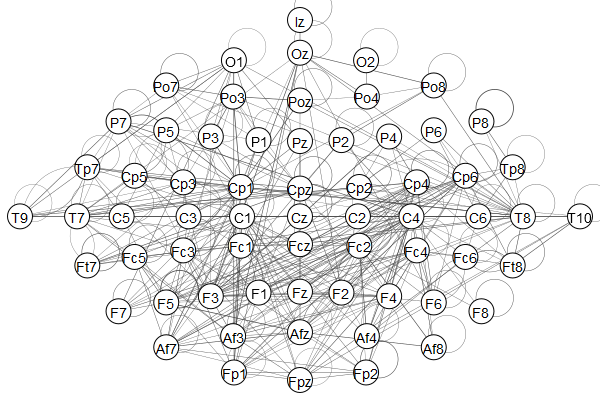
\includegraphics[width=0.7\linewidth]{../open_top_repr}
	\caption{Topographical representation of directed connectivity network for \textbf{open eyes} with density d = 0.05 (top view, nose down)}
	\label{fig:opentoprepr}
\end{figure}

\begin{figure}
	\centering
	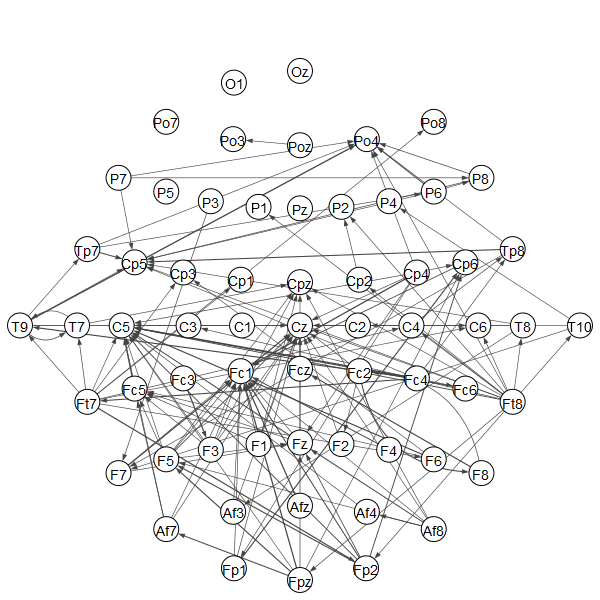
\includegraphics[width=0.7\linewidth]{../closed_top_repr}
	\caption{Topographical representation of directed connectivity network for \textbf{closed eyes} with density d = 0.05 (top view, nose down)}
	\label{fig:closedtoprepr}
\end{figure}

\section{\label{sec:level1}Graph Theory Indices}
\subsection{\label{sec:level2}Global and Local Indices}

We calculated basic indexes - both global and local - regarding the graphs generated with the techniques written above. In Figure \ref{fig:summary2} it is listed a summary that refers to binary networks. We also computed their respective weighted analogous that it is not shown in this report (for details see the attached material: \verb|main.html|).

\begin{figure}
	\centering
	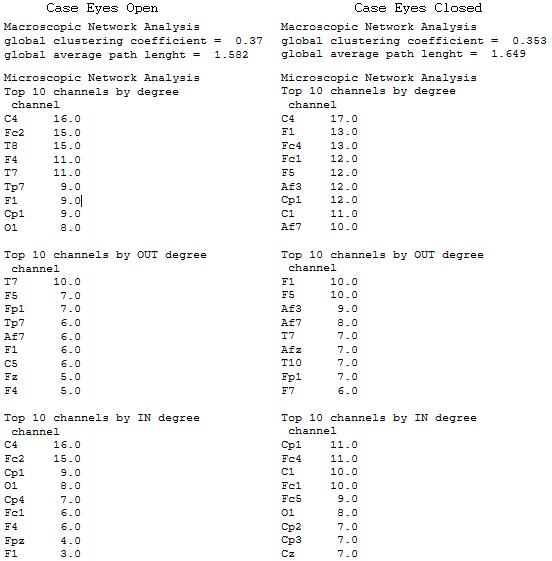
\includegraphics[width=1\linewidth]{../summary_2}
	\caption[didascalia breve]{Summary of binary global and local graph indices (top ten channels are listed) for both case studies.}
	\label{fig:summary2}
\end{figure}

\begin{figure}
	\centering
	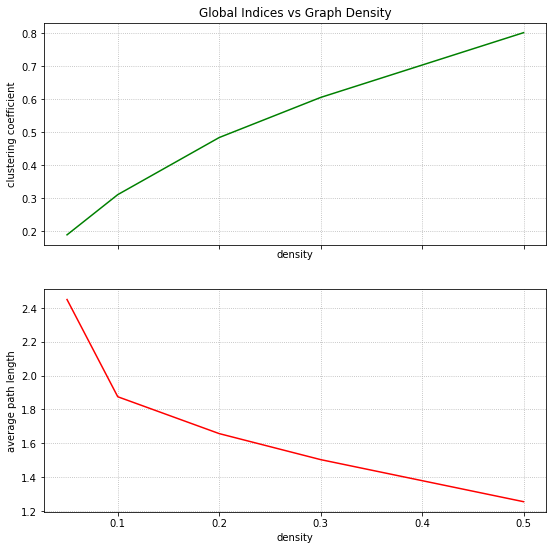
\includegraphics[width=0.5\linewidth]{../global_indices_wrt_density}
	\caption{With increasing density, we shall see that the global clustering coefficient is positively related to the density of the graph. This is expected, since the clustering coefficient is a measure of the the degree to which nodes in the graph generally tend to cluster together: when the density increases the average degree of the graph increases and as a result, it is more likely that neighbours of any given node are neighbours with each other.\\ At the same time, the more dense is a network, the more likely it is to find a shorter path that connects any two given nodes, and this gives the intuition why to higher densities correspond lower average shortest paths.}
	\label{fig:globalindiceswrtdensity}
\end{figure}



\subsection{\label{sec:level2}Small World Index}

Duncan Watts and Steven Strogatz \cite{WattsDuncan} found that graphs can be classified according to two important global indexes:

\begin{itemize}
	\item clustering coefficient
	\item average shortest path
\end{itemize}

Empirical evidence shows that many real world systems appear to be in the middle, in the sense that they share with regular networks the fact that they have an high clustering coefficient (not true for random networks), but on the other hand on these graphs, it can take only a few steps to reach, from one source, whatever target - the latter being a characteristic of random networks and not of lattices.

Watts and Strogatz measured that in fact many real-world networks have a small average shortest path length but also a clustering coefficient significantly higher than expected by random chance.

Small world networks can be considered as a trade off between two limiting topologies\cite{smallBarth}: the regular lattice, and the random graph.

We consider a graph to be a \textit{small world network} when

\begin{itemize}
	\item for any given node, neighbours of that node are likely to be connected to each other (read: high clustering coefficient)
	\item the average distance L between two nodes (average shortest path) scales as the logarithm of the number of nodes in the network: $L \sim \log N$
	
\end{itemize}

Several indexes have been proposed to measure how much a given graph satisfies these requirements\cite{smallWiki} and we will focus our attention on the small world index - \textit{SWI}. It is defined\cite{swi} as follows:

\begin{equation}
	\text{SWI} = \frac{L-L_l}{L_r-L_l} \times \frac{C-C_r}{C_l-C_r}
\end{equation}

where $C$ and $ L $ denote the clustering coefficient and average path length respectively of the actual network;  $C_r$ and $ L_r $ refer to an equivalent random network with same degree distribution, $C_l$ and $ L_l $ refer to an equivalent lattice network with same degree distribution.

Like Telesford et al \cite{smallTelesford}, we created equivalent random graphs by assigning an edge to a node pair with uniform probability while maintaining the degree distribution of the original graph\cite{maslov}, as well as using a modified version of the “latticization” algorithm\cite{sporns} found in the Brain Connectivity Toolbox\cite{bct} - we actually used \verb|bctpy|\cite{bctpy}, the Python version of the Brain Connectivity Toolbox (natively in `MATLAB`).\\

Regarding the estimation of $L_r$ and $ C_r $, since by definition they are obtained after the generation of a random network, we performed a bootstrap procedure so as to get their average value. Unfortunately, it has not been possible to sample the randomized network a lot of times because the implementation of the algorithm was not optimal time-wise. \\

We found
\[ \text{SWI} =  -0.257 \text{\quad for the EO case}\]
\[ \text{SWI} =  0.665 \text{\quad for the EC case}\]

We actually doubt these results because of the aforementioned low number of simulations, and for the negative index we received as an output in the EO condition.

\section{\label{sec:level1}Motif Analysis}

Roughly speaking, motifs in a given network are induced sub-graphs which are recurrent and statistically significant: in other words, they appear with a higher frequency than expected in 'similar' random networks.\\

Let $G$ be a network, and $G_k$ one of its own sub-networks composed by $k$ nodes. If we count how many times $G_k$ appears in $G$ for some $k$, we obtain something really analogous to a frequency spectrum, that can give a description about the basic building blocks of the net.\\

We can immediately guess that the action of counting how many times a given $G_k$ occurs in $G$ is highly computationally expensive (note also that the cardinality of the set $\{ G_k \text{ for k} \in \mathbb{N\} }$ grows exponentially with $k$). That's why one usually concentrate just on sub-graphs of size $k = 3, 4$.\\

To be more formal, we consider an induced sub-graph $G_k$ of $G$ to be a \textbf{motif} (an over represented sub-graph) if, for some set of parameters {p, U, D, N} these three requirements are satisfied:

\begin{itemize}
	\item[1] $\mathbb{P}(f_{rand}(G_k) > f_{original}(G_k)) < p$
	\item[2] $f_{original}(G_k) > U$
	\item[3] $f_{original}(G_k)- f_{rand}(G_k)>D f_{rand}(G_k)$
\end{itemize}

A $Z$ score can be assigned to each sub-graph such that

\begin{equation}
	Z = \frac{f_{original}(G_k) - <f_{rand}(G_k)>}{s(f_{rand}(G_k))}
\end{equation}

where $s(\cdot)$ is the sample standard deviation. 
Another important feature due to its interpretation in many case studies is the \textbf{anti-motif} : an induced sub-graph that satisfies the following requirements:

\begin{itemize}
	\item[1] $\mathbb{P}(f_{rand}(G_k) < f_{original}(G_k)) < p$
	\item[2] $f_{original}(G_k)- f_{rand}(G_k) < D f_{rand}(G_k)$
\end{itemize}

To perform motif analysis (i.e. to find motifs and anti-motifs in our network), we make use of the software \verb|mfinder| version 1.2\cite{mfinder}.

It has not a graphical interface, and we must use the terminal, running the following command:\\

\verb|mfinder1.2 ./data/motifAnalysis_CLOSED.txt |\\

\verb|-s 3 -r 1500 -nu -ospmem 36|\\

Here is the description of the flag commands we used:
\begin{itemize}
	\item[] \verb|-s| is the desired sub-graph size
	\item[] \verb|-r| is the number of random networks to be generated
	\item[] \verb|-nu| ignores uniqueness threshold
	\item[] \verb|-ospmem| outputs members of a list of a specific sub-graph
\end{itemize}

In our case we generated r =1000 random networks searching for the motif with id=36 which corresponds to the triad schema (s = 3) $ A\rightarrow B \leftarrow C $. Ignoring the uniqueness threshold we obtain the desired results about the pattern appearance in our graph as well as the random generated graphs.\\

The software outputs a table with some statistics regarding the candidate motifs that are repeated both in the randomized and our connections involved in the configured network.

By examining the frequency (z-score) and the statistical significance (p-value) of each candidate we chose as motifs all the candidates with $ p \leq 0.001 $ and $ Z \geq 3$, and as anti-motifs the sub-graphs with $ p \geq 0.99 $ and $ Z \leq -3$.

Results are shown in Table \ref{table:motif-analysis}.\\

\begin{table}[]
	\centering
	\begin{tabular}{llllllll}
		\multicolumn{4}{c}{Case Eyes Open} & \multicolumn{4}{c}{Case Eyes Closed} \\
		id & frequency & z-score & p-value & id & frequency & z-score & p-value \\
		38& 86 & 4.37 & 0.0001 &  36& 2559 & -6.10 & 1.000 \\
		108& 33  &3.44  & 0.0001 &  &  &  & \\
		6 & 42 & -6.43 & 1.000 & & & & \\
		36 & 1338 & -4.31 & 1.000 & & & & \\
		12 & 100 & -4.56 & 1.000 & & & & \\
		
	\end{tabular}
	\caption{motif-analysis}
	\label{table:motif-analysis}
\end{table}

Given the results corresponding to the motif analysis we concluded in selecting two motifs (38, 108) and  three anti-motifs (6, 36, 12) for case EO and just one anti-motif (id = 36) in case EC. Look at the Figure \ref{fig:motifswefound} to see the patterns which describe selected id.

\begin{figure}
	\centering
	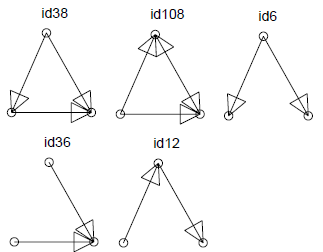
\includegraphics[width=0.7\linewidth]{../motifs_we_found}
	\caption{Dictionary of the patterns that appear as motifs or anti-motifs in our case studies}
	\label{fig:motifswefound}
\end{figure}


As we shall see the anti-motif with id=36 appears in both resting cases.

A topographical representation (Figure \ref{fig:motifopen} and Figure \ref{fig:motifclosed}) is provided for the motif with pattern $ A\rightarrow B \leftarrow C $ of the networks, considering only the connections involved in the configuration of the resting cases. Given the list of motifs with this pattern (id = 36) we draw edges with a larger width whether they connect two nodes more frequently.
\\

\begin{figure}
	\centering
	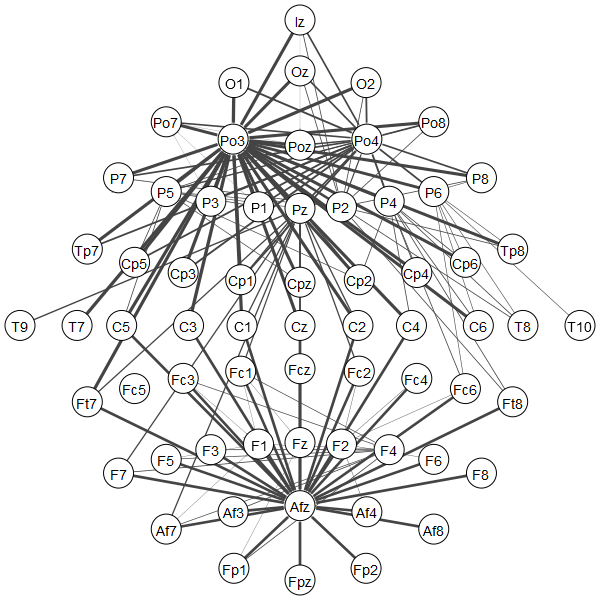
\includegraphics[width=0.7\linewidth]{../motif_open}
	\caption{Topographical representation of EO case for the motif with id = 36}
	\label{fig:motifopen}
\end{figure}

\begin{figure}
	\centering
	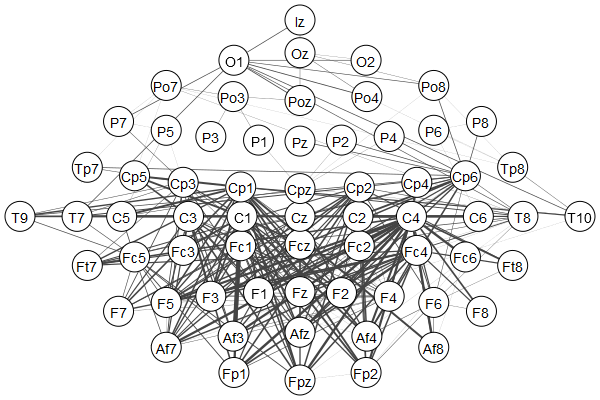
\includegraphics[width=0.7\linewidth]{../motif_closed}
	\caption{Topographical representation of EC case for the motif with id = 36}
	\label{fig:motifclosed}
\end{figure}

Regarding motif analysis, it is also possible, given a channel, to obtain the list of motifs that channel is involved with. For example, in Figure \ref{fig:motifgivenchannelpo3} we list the count of motifs that have channel \verb|Po3| as a node, which is placed in the parieto-occipital scalp region.

\begin{figure}
	\centering
	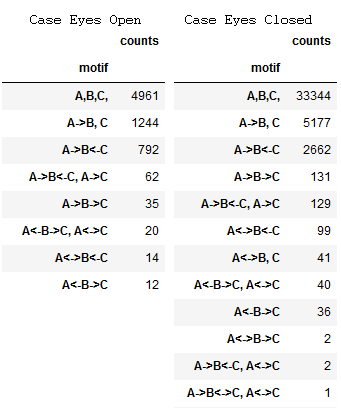
\includegraphics[width=0.7\linewidth]{../motif_given_channel_Po3}
	\caption{Motifs which involve the channel Po3 }
	\label{fig:motifgivenchannelpo3}
\end{figure}


\section{\label{sec:level1}Community Detection}

Based on the graph we have constructed before with a density equal to 5\%, we identify the community structure of the network.\\

A network is said to have community structure if the nodes of the network can be easily grouped into (potentially overlapping) sets of nodes such that each set of nodes is densely connected internally. The more general definition is based on the principle that pairs of nodes are more likely to be connected if they are both members of the same community(ies), and less likely to be connected if they do not share communities. \\

Finding an underlying community structure in a network, if it exists, appears to be important since communities allow us to create a large-scale map of a network. This is because individual communities act like meta-nodes in the entire network, fact that makes the analysis easier\cite{wikiCommu}. \\

For determining the number and composition (list of nodes and the corresponding community) of the communities, we used two methods which are based on different principles. So, in the context of community detection, we use the Louvain Method and the map equation known as Infomap. The former method is considered as a modularity-based approach in a sense that: first small communities are found by optimizing modularity locally on all nodes, then each small community is grouped into one node and the first step is repeated. The value to be optimized is modularity itself, defined as a value between -1 and 1 that measures the density of links inside communities compared to links between communities. Generally, for a weighted graph, (as in our case) modularity is defined as:

\begin{equation}
	Q = \frac{1}{2m} \sum_{ij} \left[ A_{ij} - \frac{k_i k_j}{2m} \right] \delta(c_i, c_j)
\end{equation}

where $ A_{ij} $ represents the edge weight between node i and j, $ k_i $ and $ k_j $ are the sum of the weights of the edges attached to nodes i and j respectively, $ 2m $ is the sum of all the edge weights in the graph, $ c_i $ and $ c_j $ are the communities of the nodes.\\

This method when applied is like performing a clustering algorithm that results in hierarchical refinements of the network's partitions. For this purpose we used the implementation available on the \verb|python-louvain| package which facilitates community detection of networks and builds on the \verb|igraph| package\cite{wikiLouv}.

\begin{figure}
	\centering
	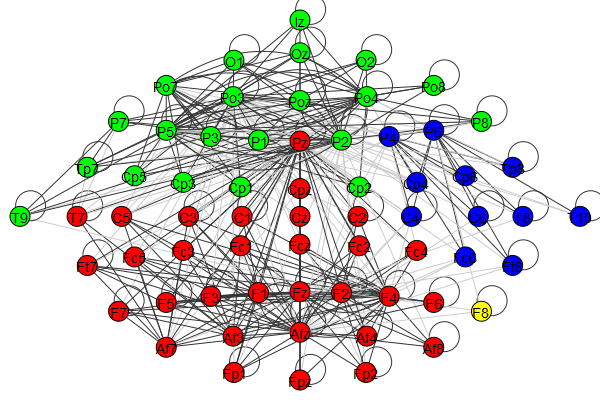
\includegraphics[width=0.7\linewidth]{../liouvain_open}
	\caption{EO case - Louvain method - Modularity based approach}
	\label{fig:liouvainopen}
\end{figure}


\begin{figure}
	\centering
	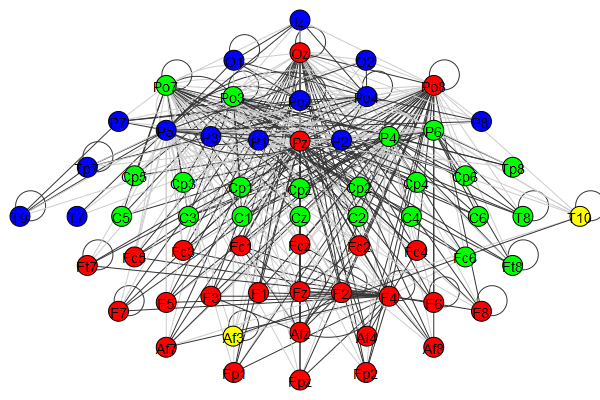
\includegraphics[width=0.7\linewidth]{../liouvain_closed}
	\caption{EC case - Louvain method - Modularity based approach}
	\label{fig:liouvainclosed}
\end{figure}

The latter approach, the application of Infomap, is mainly used for directed weighted graphs in order to identify communities according to how the information flows in the network. Huffman codes are used to give short codewords for commonly visited nodes and long codewords for rarely visited nodes. Below we cite the map equation and at the same time explain each component\cite{black}.


\begin{equation}
	L(M) = q_{\curvearrowleft} H(Q) + \sum_{i=1}^{m} p_{i \circlearrowright} H(P_i)
\end{equation}


\[ 	L(M)  \]
is the per-step description length for module partition M. That is, for module partition M of n nodes into m modules, the lower bound of the average length of
the code describing a step of the random walker.

\[ 	q_{\curvearrowleft} = \sum_{i=1}^{m} q_{i\curvearrowleft} \]

is the rate at which the index codebook is used. The per-step use rate of the index
codebook is given by the total probability that the random walker enters any of
them modules.

\[ 	H(Q) = - \sum_{i=1}^{m}\left(\frac{ q_{i\curvearrowleft}}{ q_{\curvearrowleft}} \right) \log \frac{ q_{i\curvearrowleft}}{ q_{\curvearrowleft}} \]

is the frequency-weighted average length of codewords in the index codebook.
The entropy of the relative rates to use the module codebooks measures the
smallest average codeword length that is theoretically possible.

\[ 	p_{i \circlearrowright} = \sum_{\alpha \in i} p_{\alpha} + q_{i \curvearrowright}  \]

is the rate at which the module codebook i is used, which is given by the total
probability that any node in the module is visited, plus the probability that the
random walker exits the module and the exit codeword is used.

	\[ H(P_i) = - \frac{ q_{i \curvearrowright} } { p_{i \circlearrowleft} } \log \frac{q_{i \curvearrowright}}{  p_{i \circlearrowleft} }- \sum_{\alpha \in i} \frac{ p_{\alpha }}{ p_{i \circlearrowleft} } \log \frac{ p_{\alpha}}{ p_{i \circlearrowleft} } \]

is the frequency-weighted average length of codewords in module codebook i. The
entropy of the relative rates at which the random walker exits module i and visits
each node in module i measures the smallest average codeword length that
is theoretically possible.\\

Essentially, the function and the essence of Infomap  is the minimization of the description length (Rissanen, 1978) of a random walker defined on the network through a set of processes. Consequently, we used the Infomap implementation which was available in the \verb|igraph| package.

\begin{figure}
	\centering
	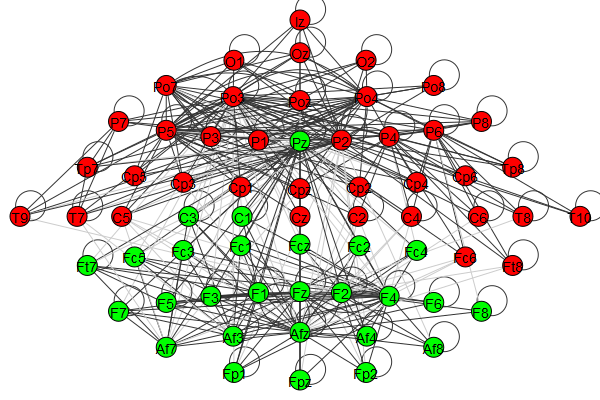
\includegraphics[width=0.7\linewidth]{../infoTheo_open}
	\caption{EO case - Infomap method - Information theory based approach}
	\label{fig:infotheoopen}
\end{figure}

\begin{figure}
	\centering
	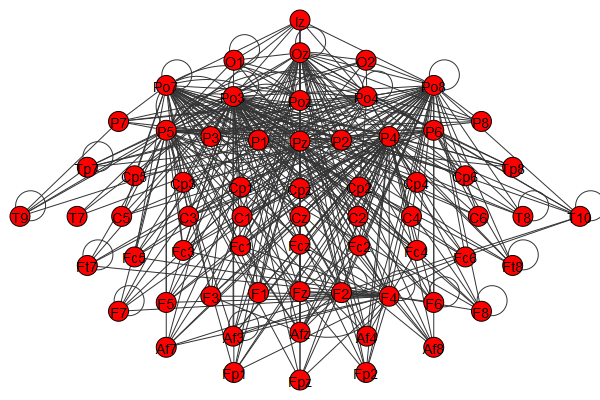
\includegraphics[width=0.7\linewidth]{../infoTheo_closed}
	\caption{EC case - Infomap method - Information theory based approach}
	\label{fig:infotheoclosed}
\end{figure}

Regarding the performance of the two previously mentioned methods we can conclude that with decreasing the network density the number of communities increases in both cases.
More specifically, with density equal to 5\%, Infomap always finds few communities regarding both resting cases. However, when a modularity-based method is applied such as the Louvain method, more communities than Infomap are found (always strictly more than one for both rest cases) for the specific average degree of our network. See Figure \ref{fig:liouvainopen} and Figure \ref{fig:liouvainclosed}.\\

These results show that with increasing network density, the Louvain Method results are not representative enough since we have each time few small communities either our graph is relatively dense or sparse. On the other hand, the Infomap method (information theory approach) detects always, even when our graph is sparse enough, a single community in the rest case where the eyes are closed (fact that intuitively makes some sense) while in the eyes-open case when applied a mid-range density (5\%-20\%) the number of computed communities varies from 1-3. See Figure \ref{fig:infotheoopen} and \ref{fig:infotheoclosed}.

 	
\section{References}
\begin{thebibliography}{}
	\bibitem{dataset} 
	Goldberger AL, Amaral LAN, Glass L, Hausdorff JM, Ivanov PCh, Mark RG, Mietus JE, Moody GB, Peng C-K, Stanley HE. PhysioBank, PhysioToolkit, and PhysioNet: Components of a New Research Resource for Complex Physiologic Signals. Circulation 101(23):e215-e220 [Circulation Electronic Pages; \url{http://circ.ahajournals.org/cgi/content/full/101/23/e215}]; 2000 (June 13). Dataset at \\
	\url{https://physionet.org/physiobank/database/eegmmidb/}\\
	
	\bibitem{pyedflib} \verb|pyedflib| module to read EDF files in \verb|python|. \url{https://github.com/holgern/pyedflib}\\
	
	\bibitem{DengfengHuang}
	\url{https://www.ncbi.nlm.nih.gov/pmc/articles/PMC4873517/}\\
	
	\bibitem{brainConEst}
	\url{https://en.wikipedia.org/wiki/Brain_connectivity_estimators}\\
	
	\bibitem{aphaFoster}
	Foster, J. J., Sutterer, D. W., Serences, J. T., Vogel, E. K., Awh, E. (2017). Alpha-Band Oscillations Enable Spatially and Temporally Resolved Tracking of Covert Spatial Attention. Psychological Science, 28(7), 929–941. \url{https://doi.org/10.1177/0956797617699167}\\
	
	\bibitem{alphaPalva}
	New vistas for $\alpha$-frequency band oscillations, Satu Palva,J. Matias Palva, Trends in Neurosciences, Elsevier, April 2007\\
	
	\bibitem{betaWiki}
	\url{https://en.wikipedia.org/wiki/Beta_wave}\\
	
	\bibitem{WattsDuncan}
	Watts, Duncan J.; Strogatz, Steven H. (June 1998). "Collective dynamics of small-world; networks";. Nature. 393 (6684): 440–442\\
	
	\bibitem{smallWiki}
	\url{https://en.wikipedia.org/wiki/Small-world_network}\\
	
	\bibitem{smallBarth}
	\url{https://arxiv.org/pdf/cond-mat/9903108.pdf}\\

	\bibitem{swi}
	Neal, Zachary P. (2017). "How small is it? Comparing indices of small worldliness". Network Science. 5 (1): 30–44. doi:10.1017/nws.2017.5. ISSN 2050-1242.\\
	
	\bibitem{smallTelesford}
	Telesford QK, Joyce KE, Hayasaka S, Burdette JH, Laurienti PJ. The ubiquity of small-world networks. Brain Connect. 2011;1(5):367-75.\\
	
	\bibitem{bct}
	\url{www.brain-connectivity-toolbox.net}\\
	
	\bibitem{bctpy}
	\url{https://github.com/aestrivex/bctpy}\\
	
	\bibitem{maslov}
	Maslov S. Sneppen K. Specificity and stability in topology of protein networks. Science. 2002;296:910–913.\\
	
	\bibitem{sporns}
	The small world of the cerebral cortex.
	Sporns O, Zwi JD
	Neuroinformatics. 2004; 2(2):145-62.\\
	
	\bibitem{wikiCommu}
	\url{https://en.wikipedia.org/wiki/Community_structure}\\
	 
	\bibitem{wikiLouv}
	\url{https://en.wikipedia.org/wiki/Louvain_Modularity}\\
	 
	\bibitem{black}
	\url{http://www.mapequation.org/assets/publications/mapequationtutorial.pdf}\\
	
	\bibitem{mfinder}
	It is available at \url{http://www.weizmann.ac.il/mcb/UriAlon/research/network-motifs}\\
	
	
\end{thebibliography}


\appendix


\section{\label{sec:level1}Extra Material}

The code that produces these results is contained inside \verb|main.html| that can be opened with a common browser. Many of the functions can be found into \verb|mvar.py|, \verb|mygraph.py|, \verb|mylib.py|.

\begin{center}
	\begin{tabular}{|c|c|} 
		\hline
		Task & Class\\ [0.5ex] 
		\hline\hline
		1.1 & mandatory\\ 
		\hline
		1.2 & A\\
		\hline
		1.3 & A\\ 
		\hline
		1.5 & C\\
		\hline
		1.6 & B\\ 
		\hline
		2.1 & mandatory\\
		\hline
		2.2 & D\\ 
		\hline
		2.4 & C\\
		\hline
		2.5 & B\\ 
		\hline
		2.7 & C\\
		\hline
		3.1 & mandatory\\ 
		\hline
		3.2 & C\\
		\hline
		3.3 & C\\
		\hline
		4.1 & mandatory\\ 
		\hline
		4.2 & B\\
		\hline
		4.3 & C \\
		\hline
	\end{tabular}	
\end{center}











\end{document}
